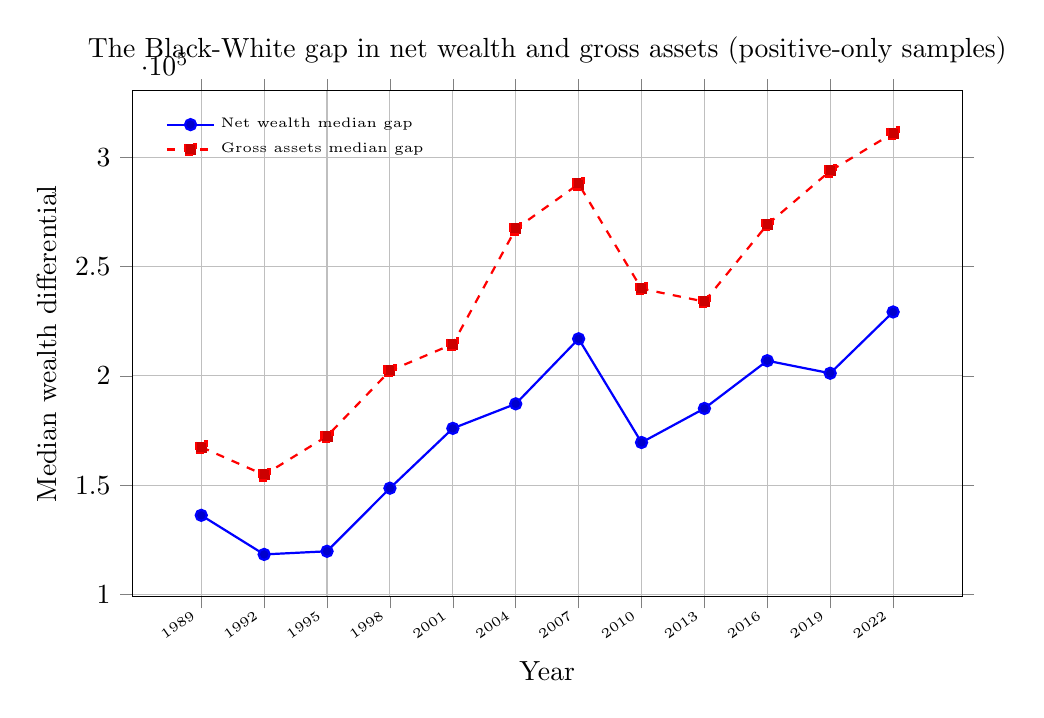
\begin{tikzpicture}
\begin{axis}[
width=\textwidth,
height=0.66\textwidth,
xlabel={Year},
ylabel={Median wealth differential},
title={The Black-White gap in net wealth and gross assets (positive-only samples)},
legend pos=north west,
legend style={font=\tiny,draw=none,fill=none,cells={anchor=west}},
grid=major,
tick align=outside,
xtick={1989,1992,1995,1998,2001,2004,2007,2010,2013,2016,2019,2022},
scaled x ticks=false,
xticklabel style={/pgf/number format/fixed,/pgf/number format/precision=0,/pgf/number format/1000 sep={},rotate=35,anchor=east,font=\tiny},
]
\addplot+[thick, blue] coordinates {(1989, 136190.89567800) (1992, 118309.46969900) (1995, 119744.85626100) (1998, 148601.66666300) (2001, 175960.73450500) (2004, 187168.66929600) (2007, 216912.51013900) (2010, 169494.88139300) (2013, 185069.92437400) (2016, 206897.97069100) (2019, 201156.89535900) (2022, 229190.00000000)};
\addlegendentry{Net wealth median gap}
\addplot+[thick, red, dashed] coordinates {(1989, 167385.45837500) (1992, 154672.53788200) (1995, 172388.46527700) (1998, 202298.83333300) (2001, 214497.65876300) (2004, 267195.26032600) (2007, 287704.11249000) (2010, 239833.20849300) (2013, 233933.98487000) (2016, 269147.43405200) (2019, 293696.25430500) (2022, 311000.00000000)};
\addlegendentry{Gross assets median gap}
\end{axis}
\end{tikzpicture}
